%-----------------------------------------------------------------------------
%
%          PHYSICS  M.S.     THESIS
%          JUSTIN A. VASEL
%
%          This began as the template offered by the University of Minnesota, 
%          but I've made a few changes here and there...  
%
%          -->  snews.tex
%
%-----------------------------------------------------------------------------


\chapter{The Supernova Early Warning System}
	\label{snews_chapter}
	\vspace{-0.2in}

	\begin{quoting}
		\noindent \large ``Vision is the art of seeing things invisible." \normalsize

		--- Jonathan Swift
	\end{quoting}

	\chapterIntro{L}{ittle is known about the behavior of a star moments from death.} Understanding of main-sequence stellar behavior is always improving thanks to a robust nuclear theory, powerful computational models, and observation. But, after a star moves off of the main sequence conditions inside are harder to predict with any confidence. Perhaps the best example of this are the moments immediately preceding and immediately following the eruptions of large stars. Computational models are always improving, but its very hard to compare them with observations because it is difficult to predict when and where a supernova will occur. 

	The possibility of using the neutrino signal as an advance warning of the photon signal was fully realized with the eruption of SN 1987a, \SI{50}{\kilo\parsec} away in the Large Magellanic Cloud. A handful of neutrino detectors at the time recorded the event. A total of 26 events were observed between Kamiokande-II, IMB, and Baksan over a period of 13 seconds, all with energies $\lesssim$ \nolinebreak \eMeV{40} (\FIG \ref{fig:SN1987curve})\cite{kii1987a,imb_1987a,baksan1987a}.

	\begin{figure}[H]
	\centering
	    \begin{tikzpicture}[scale=1.5]
	    	\pgfplotsset{every axis legend/.append style={
				at={(0.5,1.03)},
				anchor=south}}
		    \begin{axis}[xmin=0,xmax=15,ymin=0,ymax=50,title={},%
		    xlabel={Time (s)}, ylabel={Neutrino energy (MeV)},%
		    legend cell align=left, only marks, legend columns=3, legend style={/tikz/every even column/.append style={column sep=0.5cm}}]
		        \addplot[red,thick,mark=*,/pgfplots/error bars/.cd, x dir=none,y dir=both,y explicit] table[x index=0, y index=1, y error index=2] {./Chapters/Supplementary/k2.dat};
		        \addlegendentry{Kamiokande II}
		        \addplot[blue,thick,mark=square*,/pgfplots/error bars/.cd, x dir=none,y dir=both,y explicit] table[x index=0, y index=1, y error index=2] {./Chapters/Supplementary/imb.dat};
		        \addlegendentry{IMB}
		        \addplot[black,thick,mark=triangle*,/pgfplots/error bars/.cd, x dir=none,y dir=both,y explicit] table[x index=0, y index=1, y error index=2] {./Chapters/Supplementary/baksan.dat};
		        \addlegendentry{Baksan}
		    \end{axis}
	    \end{tikzpicture}
	    \caption[Observed Neutrino Spectrum From SN 1987a]{\bf Observed neutrino spectrum from SN 1987a. \rm Twenty six events were recorded by three separate experiments during a 13-second period. A scintillator detector in Mont Blanc in Italy detected a neutrino signal, but it was not coincident with the other detectors and are not thought to be associated with the supernova\cite{Arnett1989}.} \label{fig:SN1987curve}
	\end{figure}

	The Supernova Early Warning System (SNEWS)\footnote{http://snews.bnl.gov} \cite{Scholberg2008} is hoping to take advantage of the neutrino signal generated during galactic core-collapse supernovae to identify the explosion before the photon signal arrives. SNEWS is a world-wide network of neutrino detectors that will listen for that distinct neutrino signal and alert the astronomical community upon its arrival. Astronomers will only have several hours to prepare their observations. 


	%% SECTION : A WORLD-WIDE NETWORK OF NEUTRINO DETECTORS
	\section{A World-Wide Network of Neutrino Detectors}
	There are at present five neutrino observatories actively participating in SNEWS: IceCube in Antarctica, Borexino and the Large Volume Detector (LVD) in Italy, and Super-Kamiokande (Super-K) and KamLAND in Japan. HALO and a few other experiments like SNO+ in Canada and NO$\nu$A in Minnesota plan to join that list soon. A brief summary of each detector is given in \TAB \ref{table:snews_detectors}.
		\begin{figure}[H]
		\centering
		\includegraphics[width=1\textwidth]{snews_map}
		\caption[Map of Observatories Participating in SNEWS]{\bf Map of observatories participating in SNEWS. \rm At present, five observatories are actively participating (purple markers). HALO, SNO+, and NO$\nu$A plan to actively participate once their triggers are in place (red markers).}
		\label{fig:snews_map}
	\end{figure}

	The experiments share a connection to two central servers, one at Brookhaven National Laboratory (BNL) and another at the Istituto Nazionale di Fisica Nucleare in Italy, which functions as a backup in case BNL goes offline. Through automated triggering software, each experiment automatically sends an alert to the central server when it believes it detected a supernova neutrino signal. If the server receives several coincident alerts, it sends the warning out to the SNEWS membership via a PGP encrypted email. 

	\begin{table}[H]
		\centering
		\caption[Summary of SNEWS Detectors]{A summary of SNEWS-affiliated detectors and their attributes\cite{Antonioli2004}.}
		\label{table:snews_detectors}
			\begin{tabular}{lcccc}
				\toprule
				Detector & Type & Mass (kton) & Location & Status \\
				\midrule
				IceCube & H$_2$O (ice) Cherenkov & -- & Anarctica & Running \\
				Borexino & Liquid Scintillator & 0.30 & Italy & Running \\
				LVD & Liquid Scintillator & 1 & Italy & Running \\
				Super-K & H$_2$O Cherenkov 	& 32 & Japan & Running \\
				HALO & High-Z (Pb) & 0.076 & Canada & In Development \\
				SNO+ & Liquid Scintillator & 0.78 & Canada & In Development \\
				\bottomrule
			\end{tabular}
	\end{table}


	%% SECTION : THE THREE P'S
	\section{The Three P's}
	In order for SNEWS to be reliable and successful, it has to adhere to ``the three P's":

	\subsection*{Prompt}
	The prompt neutrino signal may only precede the photon signal by hours or less. It is essential that SNEWS works quickly to get the word out once the neutrino signal is detected. To achieve this, the system is automated at both the detector end and the server end. Each experiment is responsible for developing its own software triggers that alert SNEWS when a supernova candidate is detected. 

	\subsection*{Pointing}
	Knowing that a supernova is about to become visible is great. What's better is knowing where to look. Detecting the directionality of incoming neutrinos is notoriously difficult. Many neutral and charged current interactions are useless because their products are nucleons or leptons whose directions are independent of that of the neutrino. However, elastic scattering between neutrinos and electrons ($\HepProcess{\HepParticle{\Pneutrino}{}{} + \HepParticle{\Pelectron}{}{} \to \HepParticle{\Pneutrino}{}{} + \HepParticle{\Pelectron}{}{}}$), which is a neutral current process, is currently the best method because the momentum transfered to the electron points back to the direction of the incoming neutrino. Super-Kamiokande is currently the only SNEWS observatory that can provide pointing information. For a supernova at a distance of \SI{10}{\kilo\parsec} from Earth, Super-K can point with an accuracy of about \ang{7.8} if an isotropic background is present. If the background can be accounted for with neutron tagging, the accuracy improves to about \ang{3.2}\cite{Tomas2003}. Triangulation between detectors around the world is technically possible, but currently the statistics associated with interactions make it too difficult. It has been proposed that the next generation of high-statistics neutrino observatories (eg. Hyper-Kamiokande) may be able to use triangulation to determine a rough location in the sky\cite{Muhlbeier2013}.

	%\vspace{0.5in}
	\subsection*{Positive}
	\label{sec:snews_positive}

	\begin{wrapfigure}{r}{0.68\textwidth}
		\vspace{-0.9in}
		\centering
		\includegraphics[width=0.68\textwidth]{coincidence}
		\caption[SNEWS Rate of Accidental Alerts]{\bf SNEWS rate of accidental alerts.\rm The average interval between false-alarms is modeled to first order as a Poisson process parameterized by the number of required coincidences in a 10 second window and the number of active experiments\cite{Antonioli2004}.}
		\label{fig:coincidence}
		\vspace{0.0in}
	\end{wrapfigure}


	To ensure that a SNEWS alert is taken seriously, the false-alarm rate of SNEWS must be very low. SNEWS aims for a false-alarm rate of fewer than one per century. To achieve this, SNEWS requires that each experiment has a false-alarm rate of less than once per week and that at least two detectors send an alert within ten seconds of each other. This 2-fold coincidence between detectors ensures the once-per-century threshold can be achieved, but only with three actively participating experiments. If more than three experiments are participating, the coincidence between detectors must be at least 3-fold if each detector is to maintain a once-per-week false alarm rate pre-coincidence (\FIG \ref{fig:coincidence}).


	%% SECTION : ALERTING THE ASTRONOMICAL COMMUNITY
	\section{Alerting the Astronomical Community}
	Each experiment participating in SNEWS is responsible for implementing an automated supernova trigger with the certainty detailed in the previous section. When an experiment's trigger is activated, the experiment will send an alarm datagram to the ``coincidence server'' in Brookhaven National Laboratory. The coincidence server then scrutinizes the datagram and listens for coincident alarms from other experiments. A 2-fold coincidence within 10 seconds is required to trigger an automated alert. If the coincidence criterion is not met, an individual alert can be sent if the experiment confirms the signal is not noise, otherwise the datagram is discarded and SNEWS returns to waiting for alarms (\FIG \ref{fig:flowchart}).

	If the coincidence criterion is met, then SNEWS will issue either a GOLD or SILVER alert, depending the quality of the alarm received. Besides coincidence, for a GOLD alarm to be issued at least two of the experiments involved must be a physically separated laboratories. Furthermore two or more of the alarms received must be flagged as ``GOOD''. This means that the alarm was received while the experiments were operating under normal conditions, rather than operating during maintenance or callibrtion, for example. Finally, at least two of the experiments involved must have had an acceptable false-alarm rate of \SI[mode=text]{1}{week^{-1}} during the past time intervals $\{T_i\} = \{\SI[mode=text]{10}{minutes}, \SI[mode=text]{1}{hour}, \SI[mode=text]{10}{hours}, \SI[mode=text]{1}{day}, \SI[mode=text]{3}{days}, \SI[mode=text]{1}{week}, \SI[mode=text]{1}{month}\}$.

	If a coincident alarm fails to meet all these criteria, the alert will be demoted to SILVER. A SILVER alert only gets issued to experimenters, not the general public. In this case experimenters must personally check their data and decide if it is a suitable supernova candidate. If so, the experimenters send an OVERRIDE packet to the server and SNEWS promotes the alert to GOLD. A GOLD alert is issued to experimenters and the public. Again, the experimenters must hand-check their data. If through this checking it is discovered that it was a false alarm, a retraction is issued to the mailing lists and on the SNEWS web page.

	\begin{figure}[H]
		\centering
		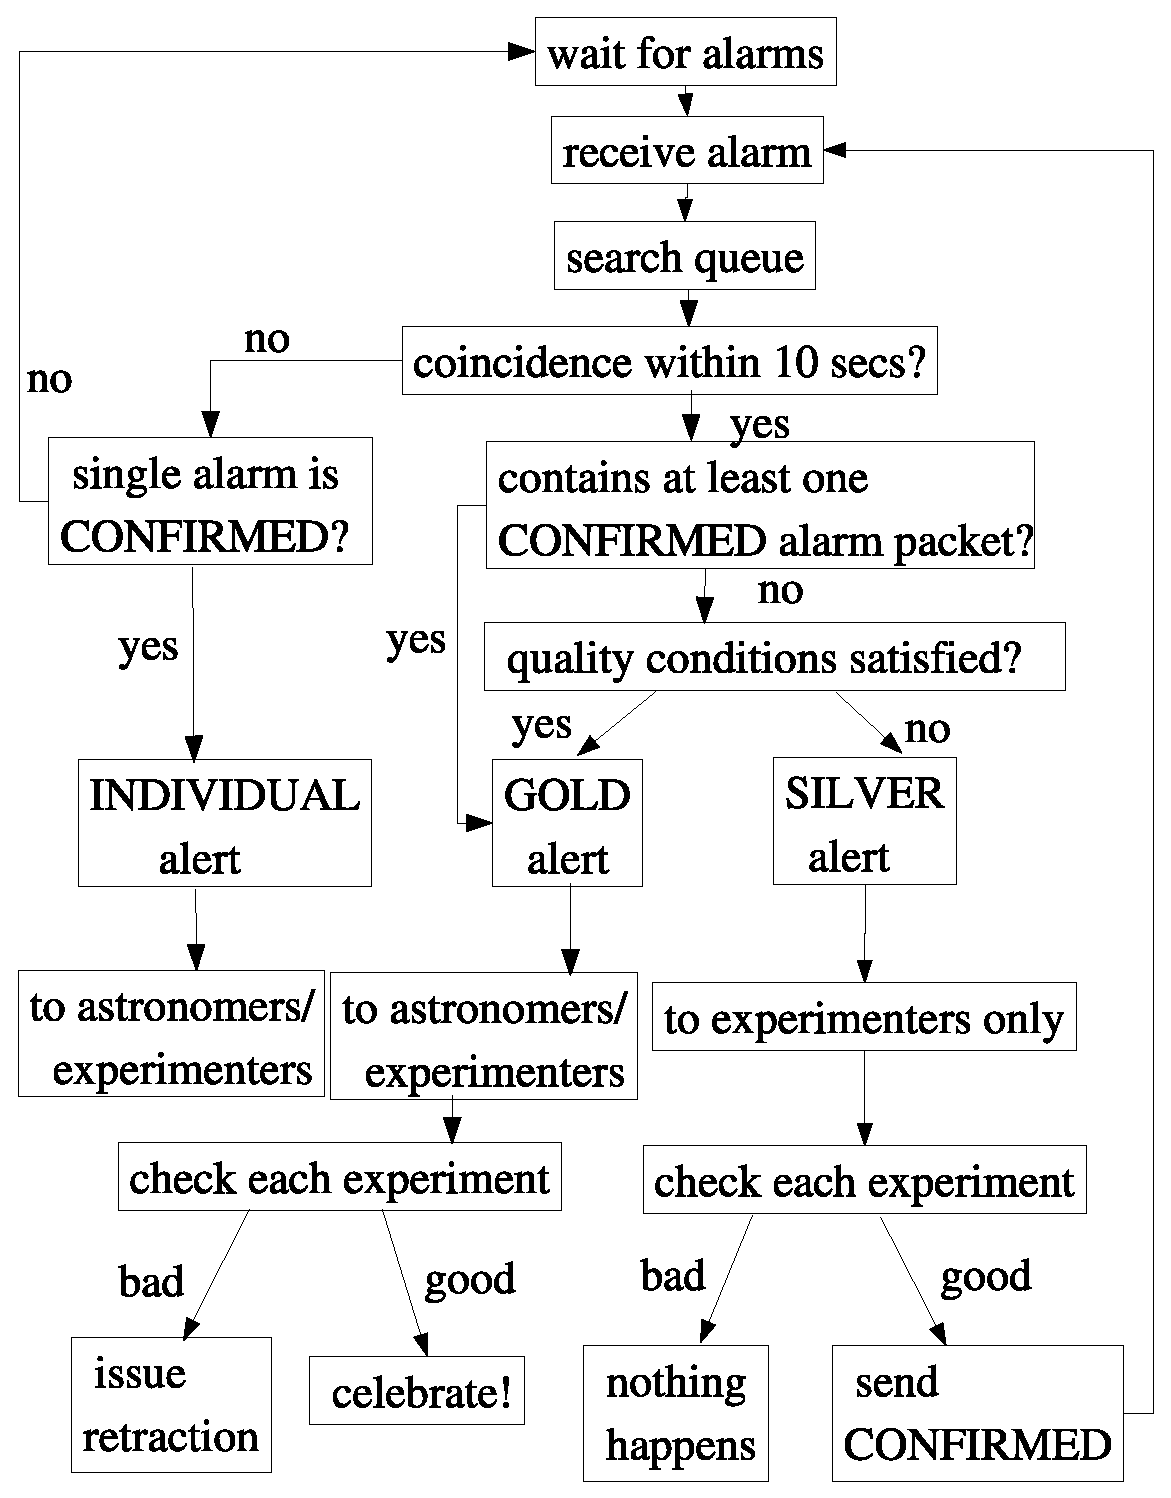
\includegraphics[width=0.68\textwidth]{snews_flowchart}
		\caption[SNEWS Flowchart]{\bf SNEWS alert flowchart\rm\cite{Scholberg2008}. This algorithm runs on the SNEWS coincidence server at Brookhaven National Laboratory, and discriminates against alarms to determine their candidacy as a supernova event.}
		\label{fig:flowchart}
	\end{figure}

	The intended subscribers of the SNEWS service are astronomers, although anybody who would like to receive alerts can sign up.\footnote{Join the mailing list: http://snews.bnl.gov/alert.html} An alert sent to the community will contain information about the time of the event and an approximate location in the sky bounded by an error box. This pointing information may not be included with any alert; it depends on which experiments can provide such information and whether they were involved in the coincidence. The neutrino detectors are the ear, but the optical telescopes are the eyes. The amateur astronomers---being skilled, enthusiastic, and well-equipped---are well suited for this task.

	In 2003, a test alert was issued to observe the system in action. The asteroid Vesta was selected as the test target and the position with a 13 degree uncertainty was distributed to the mailing list. Amateur astronomers world-wide submitted 83 responses, of which six had successfully identified the target\cite{Antonioli2004}. The system worked.

%-----------------------------------------------------------------------------
%-----------------------------------------------------------------------------